\documentclass[journal]{IEEEtran}
\usepackage[a5paper, margin=10mm]{geometry}
\usepackage{tfrupee} % Include tfrupee package


\setlength{\headheight}{1cm} % Set the height of the header box
\setlength{\headsep}{0mm}     % Set the distance between the header box and the top of the text


\setlength{\intextsep}{10pt} % Space between text and floats

\makeindex


\usepackage{cite}
\usepackage{amsmath,amssymb,amsfonts,amsthm}
\usepackage{algorithmic}
\usepackage{graphicx}
\usepackage{textcomp}
\usepackage{xcolor}
\usepackage{txfonts}
\usepackage{listings}
\usepackage{enumitem}
\usepackage{mathtools}
\usepackage{gensymb}
\usepackage{comment}
\usepackage[breaklinks=true]{hyperref}
\usepackage{tkz-euclide} 
\usepackage{listings}
\usepackage{multicol}
\usepackage{xparse}
\usepackage{color}                                            
\usepackage{array}                                          
\usepackage{longtable}                                     
\usepackage{calc}                                             
\usepackage{multirow}                                       
\usepackage{hhline}                                           
\usepackage{ifthen}                                           
\usepackage{lscape}
\usepackage{tabularx}
\usepackage{array}
\usepackage{float}
\usepackage{ar}
\usepackage{gvv}
\usepackage[version=4]{mhchem}



\newtheorem{theorem}{Theorem}[section]
\newtheorem{problem}{Problem}
\newtheorem{proposition}{Proposition}[section]
\newtheorem{lemma}{Lemma}[section]
\newtheorem{corollary}[theorem]{Corollary}
\newtheorem{example}{Example}[section]
\newtheorem{definition}[problem]{Definition}
\newcommand{\BEQA}{\begin{eqnarray}}
\newcommand{\EEQA}{\end{eqnarray}}

\theoremstyle{remark}

\begin{document}
\bibliographystyle{IEEEtran}
\onecolumn

\title{METALLURGY ENGINEERING (MT)}
\author{GATE 2024 Questions\\EE25BTECH11027-INDHIRESH S}
\maketitle

\renewcommand{\thefigure}{\theenumi}
\renewcommand{\thetable}{\theenumi}

\section*{General Aptitude}
\subsection*{Q.1 - Q.5 Carry ONE mark Each}
\begin{enumerate}
\item If `$\rightarrow$` denotes increasing order of intensity, then the meaning of the words [dry $\rightarrow$ arid $\rightarrow$ parched] is analogous to [diet $\rightarrow$ fast $\rightarrow$ \_]. \hfill{\brak{\text{GATE MT 2024}}}\\
Which one of the given options is appropriate to fill the blank?
\begin{multicols}{4}
\begin{enumerate}
\item starve
\item reject
\item feast
\item deny
\end{enumerate}
\end{multicols}

\item If two distinct non-zero real variables $x$ and $y$ are such that $(x+y)$ is proportional to $(x-y)$ then the value of $\frac{x}{y}$ \hfill{\brak{\text{GATE MT 2024}}}
\begin{enumerate}
\item depends on $xy$
\item depends only on $x$ and not on $y$
\item depends only on $y$ and not on $x$
\item is a constant
\end{enumerate}

\item Consider the following sample of numbers:\\
9, 18, 11, 14, 15, 17, 10, 69, 11, 13. \hfill{\brak{\text{GATE MT 2024}}}\\
The median of the sample is
\begin{multicols}{4}
\begin{enumerate}
\item 13.5
\item 14
\item 11
\item 18.7
\end{enumerate}
\end{multicols}

\item The number of coins of $\text{\rupee} 1, \text{\rupee}25 ,\; \text{and} \;\text{\rupee}10$  denominations that a person has are in the ratio 5:3:13. Of the total amount, the percentage of money in 25 paise coins is \hfill{\brak{\text{GATE MT 2024}}}
\begin{multicols}{2}
\begin{enumerate}
\item 21\%
\item $14\frac{2}{7}\%$
\item 10\%
\item 30\%
\end{enumerate}
\end{multicols}

\item For positive non-zero real variables $p$ and $q$, if 
\begin{align}
    \log(p^2+q^2) = \log p + \log q + 2\log 3
\end{align}
, then, the value of $\frac{p^4+q^4}{p^2q^2}$ is \hfill{\brak{\text{GATE MT 2024}}}
\begin{multicols}{4}
\begin{enumerate}
\item 79
\item 81
\item 9
\item 83
\end{enumerate}
\end{multicols}
\end{enumerate}

\subsection*{Q.6 - Q.10 Carry TWO marks Each}
\begin{enumerate}[resume]
\item In the given text, the blanks are numbered (i)-(iv). Select the best match for all the blanks. \hfill{\brak{\text{GATE MT 2024}}}\\
\textit{Steve was advised to keep his head \underline{\hspace{0.5cm}}(i)\underline{\hspace{0.5cm}} before heading \underline{\hspace{0.5cm}}(ii)\underline{\hspace{0.5cm}} to bat; for, while he had a head \underline{\hspace{0.5cm}}(iii)\underline{\hspace{0.5cm}} his shoulders, he could only do so with a cool head.} 

\begin{enumerate}
    \item (i) down, (ii) down, (iii) on
    \item (i) on, (ii) down, (iii) for
    \item (i) down, (ii) out
    \item (i) on
\end{enumerate}

\item A rectangular paper sheet of dimensions 54 cm $\times$ 4 cm is taken. The two longer edges of the sheet are joined together to create a cylindrical tube. A cube whose surface area is equal to the area of the sheet is also taken. Then, the ratio of the volume of the cylindrical tube to the volume of the cube is \hfill{\brak{\text{GATE MT 2024}}}
\begin{multicols}{4}
\begin{enumerate}
\item $1/\pi$
\item $2/\pi$
\item $3/\pi$
\item $4/\pi$
\end{enumerate}
\end{multicols}

\item The pie chart presents the percentage contribution of different macronutrients to a typical 2,000 kcal diet of a person. The typical energy density (kcal/g) of these macronutrients is given in the table. The total fat (all three types), in grams, this person consumes is \hfill{\brak{\text{GATE MT 2024}}}
\begin{figure}[H]
    \centering
    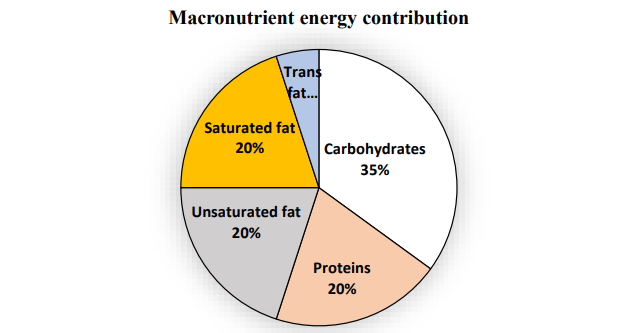
\includegraphics[width=0.6\columnwidth]{figs/Q.8.png}
    \caption\centering{MACRONUTRIENT ENERGY CONTRIBUTION}
    \label{fig:placeholder}
\end{figure}
\begin{center}
\begin{tabular}{|l|l|}
\hline
\textbf{Macronutrient} & \textbf{Energy density (kcal/g)} \\
\hline
Carbohydrates & 4 \\
Proteins & 4 \\
Unsaturated fat & 9 \\
Saturated fat & 9 \\
Trans fat & 9 \\
\hline
\end{tabular}
\end{center}
\begin{multicols}{4}
\begin{enumerate}
\item 44.4
\item 77.8
\item 100
\item 3,600
\end{enumerate}
\end{multicols}

\item A rectangular paper of $20\;cm \times 8$ cm is folded 3 times. Each fold is made along the line of symmetry, which is perpendicular to its long edge. The perimeter of the final folded sheet (in cm) is \hfill{\brak{\text{GATE MT 2024}}}
\begin{multicols}{4}
\begin{enumerate}
\item 18
\item 24
\item 20
\item 21
\end{enumerate}
\end{multicols}

\item The least number of squares to be added in the figure to make AB a line of symmetry is \hfill{\brak{\text{GATE MT 2024}}}
\begin{figure}[H]
    \centering
    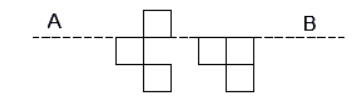
\includegraphics[width=0.4\columnwidth]{figs/Q.10.png}
    \caption\centering{FIGURE}
    \label{fig:placeholder}
\end{figure}
\begin{multicols}{4}
\begin{enumerate}
\item 6
\item 4
\item 5
\item 7
\end{enumerate}
\end{multicols}
\end{enumerate}

\section*{Metallurgical Engineering}
\subsection*{Q.11 - Q.35 Carry ONE mark Each}
\begin{enumerate}[resume]
\item If $X_1$ and $X_2$ are independent normally distributed random variables with means $\mu_1$ and $\mu_2$, and variances $\rho_1$ and $\rho_2$, respectively, then the combination $X = X_1 + X_2$ has mean $\mu$ and variance $\rho$ such that \hfill{\brak{\text{GATE MT 2024}}}
\begin{enumerate}
\item $\mu = \mu_1 + \mu_2$ and $\rho = \rho_1 + \rho_2$
\item $\mu^2 = \mu_1^2 + \mu_2^2$ and $\rho = \rho_1 + \rho_2$
\item $\mu = \mu_1 + \mu_2$ and $\rho^2 = \rho_1^2 + \rho_2^2$
\item $\mu^2 = \mu_1^2 + \mu_2^2$ and $\rho^2 = \rho_1^2 + \rho_2^2$
\end{enumerate}

\item Which one of the following is the Taylor series expansion of $\ln(\frac{1+x}{1-x})$ about the origin for $|x|<1$? x is a real number \hfill{\brak{\text{GATE MT 2024}}}
\begin{multicols}{2}
\begin{enumerate}
\item $x - \frac{x^2}{2} + \frac{x^3}{3} - \dots$
\item $2(x - \frac{x^2}{2} + \frac{x^3}{3} - \dots)$
\item $x + \frac{x^3}{3} + \frac{x^5}{5} + \dots$
\item $2(x + \frac{x^3}{3} + \frac{x^5}{5} + \dots)$
\end{enumerate}
\end{multicols}

\item Consider the normal (Gaussian) distributions a, b, c shown in the figure. $\sigma_p$ and $\mu_p$ are the standard deviation and mean of a distribution p, respectively, and the means are positive. Which one of the following deductions is correct? \hfill{\brak{\text{GATE MT 2024}}}
\begin{figure}[H]
    \centering
    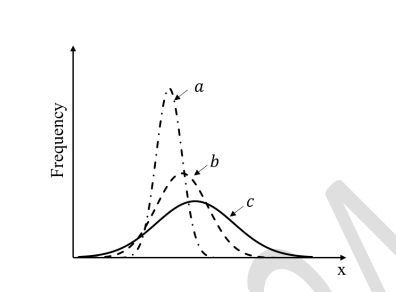
\includegraphics[width=0.4\columnwidth]{figs/Q.13.png}
    \caption\centering{FIGURE}
    \label{fig:placeholder}
\end{figure}
\begin{multicols}{2}
\begin{enumerate}
\item $\sigma_a < \sigma_b < \sigma_c$
\item $\sigma_a > \sigma_b > \sigma_c$
\item $\mu_a = \mu_b = \mu_c$
\item $\mu_a > \mu_b > \mu_c$
\end{enumerate}
\end{multicols}
\item If in an A-B solid solution, the activity and mole fraction of A are given by $a_A$ and $X_A$, respectively, then the activity coefficient of A is given by \hfill{\brak{\text{GATE MT 2024}}}
\begin{multicols}{4}
\begin{enumerate}
\item $\frac{a_A}{X_A}$
\item $\frac{X_A}{a_A}$
\item $a_A X_A$
\item $a_A X_A^2$
\end{enumerate}
\end{multicols}

\item As shown in the figure, two rods of different metals of equal lengths, $L/2$, diameter $d$ ($d \ll L$), and constant thermal conductivities $k_1$ and $k_2$ (with $k_1 > k_2$) are connected perfectly (i.e., zero interface thermal resistance).
\begin{figure}[H]
    \centering
    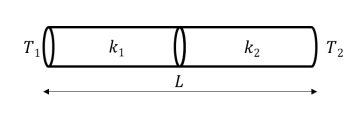
\includegraphics[width=0.5\columnwidth]{figs/Q.15(1).png}
    \caption\centering{FIGURE}
    \label{fig:placeholder}
\end{figure}
The left and right ends of the connected rod are maintained at temperatures $T_1$ and $T_2$ ($T_1 > T_2$). Assume that the rods are insulated from the environment, apart from the two flat ends. Which one of the following graphs represents the temperature distribution at steady-state? The thickest line shows the temperature profile. The horizontal axis shows the distance from the left end of the rod to the right and the vertical axis denotes temperature. \hfill{\brak{\text{GATE MT 2024}}}
\begin{figure}[H]
    \centering
    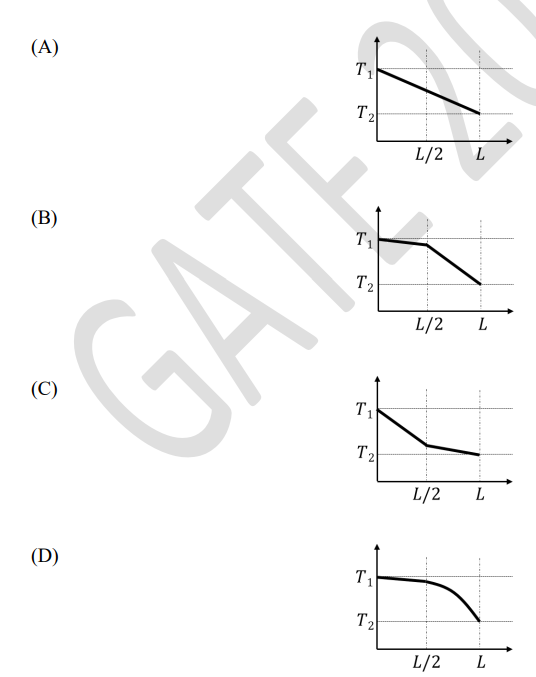
\includegraphics[width=0.7\columnwidth]{figs/Q.15(2).png}
    \caption\centering{GRAPHS}
    \label{fig:placeholder}
\end{figure}



\item Match the laws listed in Column I with the corresponding material properties listed in Column II. \hfill{\brak{\text{GATE MT 2024}}}
\begin{center}
\begin{tabularx}{0.8\textwidth}{lX}
\textbf{Column I} & \textbf{Column II} \\
(P) Hooke's law & (1) Thermal conductivity \\
(Q) Fick's law & (2) Young's modulus \\
(R) Fourier's law & (3) Permeability \\
(S) Darcy's law & (4) Diffusivity \\
\end{tabularx}
\end{center}
\begin{multicols}{2}
    

\begin{enumerate}
\item P-2, Q-1, R-4, S-3
\item P-4, Q-3, R-1, S-2
\item P-2, Q-4, R-1, S-3
\item P-4, Q-3, R-2, S-1
\end{enumerate}
\end{multicols}

\item Wet high intensity magnetic separators (WHIMS) are used to concentrate \hfill{\brak{\text{GATE MT 2024}}}
\begin{enumerate}
\item fine ($< 75\; \mu m$) paramagnetic minerals.
\item coarse ($> 75\; \mu m$) ferromagnetic minerals.
\item coarse ($> 75\; \mu m$) paramagnetic minerals.
\item fine ($< 75\; \mu m$) ferromagnetic minerals.
\end{enumerate}

\item Which one of the following reagents is NOT used in froth flotation process? \hfill{\brak{\text{GATE MT 2024}}}
\begin{multicols}{2}
\begin{enumerate}
\item Lixiviants
\item Collectors
\item Activators
\item Depressants
\end{enumerate}
\end{multicols}

\item Which one of the following reactions is the Boudouard's reaction? Given: (s): solid,(l):liquid, (g): gas \hfill{\brak{\text{GATE MT 2024}}}
\begin{enumerate}
\item $C(s) + H_2O(l) \rightarrow H_2(g) + CO(g)$
\item $C(s) + O_2(g) \rightarrow CO_2(g)$
\item $C(s) + CO_2(g) \rightarrow 2CO(g)$
\item $2C(s) + O_2(g) \rightarrow 2CO(g)$
\end{enumerate}

\item Which one of the following processes is NOT related to the extraction and refining of titanium from ilmenite ore? \hfill{\brak{\text{GATE MT 2024}}}
\begin{multicols}{2}
\begin{enumerate}
\item Pidgeon's process
\item Sorel process
\item Van Arkel process
\item Kroll's process
\end{enumerate}
\end{multicols}

\item Which one of the following is the correct statement about the industrial production of aluminium from pure dry alumina by Hall-Héroult electrolytic reduction? \hfill{\brak{\text{GATE MT 2024}}}
\begin{enumerate}
\item Cell is operated at a high voltage (220 to 240 V) with a very low current density.
\item Cell is operated at a low voltage (5 to 7 V) with a very low current density.
\item Cell is operated at a high voltage (220 to 240 V) with a very high current density.
\item Cell is operated at a low voltage (5 to 7 V) with a very high current density.
\end{enumerate}

\item Which one of the following schematics represents the variation of the rate of nucleation of solid from a pure liquid metal as a function of undercooling ($\Delta T = T_m - T$, where $T_m$ and $T$ are the freezing temperature and the liquid temperature, respectively)? \hfill{\brak{\text{GATE MT 2024}}}
\begin{figure}[H]
    \centering
    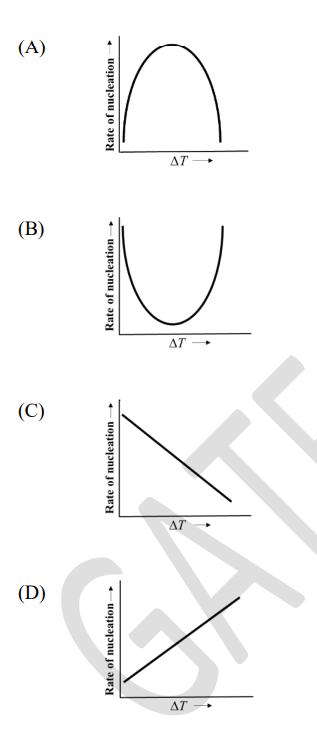
\includegraphics[width=0.4\columnwidth]{figs/Q.22.png}
    \caption\centering{SCHEMATIC DIAGRAMS}
    \label{fig:placeholder}
\end{figure}

\item Which one of the following crystal structure changes occurs during the transformation of mild steel from austenite to martensite? \hfill{\brak{\text{GATE MT 2024}}}
\begin{enumerate}
\item Face centered cubic to body centered cubic
\item Face centered cubic to body centered tetragonal
\item Body centered cubic to body centered tetragonal
\item Body centered tetragonal to face centered cubic
\end{enumerate}

\item The figure shows a dislocation loop (shown by the solid circle), whose Burgers vector is b (shown by the horizontal arrow inside the dislocation loop). Identify the nature of the dislocation segment at locations p, q and r. The dash-dot lines show the horizontal and vertical diameters of the loop, and the arrow along the dislocation loop indicates the line vector. \hfill{\brak{\text{GATE MT 2024}}}
\begin{figure}[H]
    \centering
    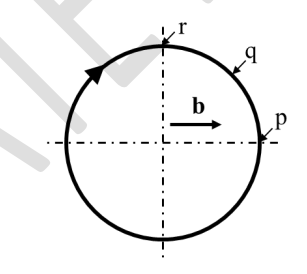
\includegraphics[width=0.3\columnwidth]{figs/Q.24.png}
    \caption\centering{DISLOCATION LOOP}
    \label{fig:placeholder}
\end{figure}
\begin{enumerate}
\item p: pure edge, q: mixed, r: pure screw
\item p: pure edge, q: pure screw, r: pure edge
\item p: pure screw, q: mixed, r: pure screw
\item p: pure screw, q: pure edge, r: pure screw
\end{enumerate}

\item Match the concepts listed in Column I with the phenomena listed in Column II. \hfill{\brak{\text{GATE MT 2024}}}
\begin{center}
\begin{tabular}{ll}
\textbf{Column I} & \textbf{Column II} \\
P. Peierls-Nabarro stress & 1. Yield point phenomenon \\
Q. Cottrell's atmosphere & 2. Fatigue \\
R. Paris law & 3. Dislocation glide \\
S. Considère's criterion & 4. Onset of necking \\
\end{tabular}
\end{center}
\begin{enumerate}
\item P-1, Q-2, R-3, S-4
\item P-4, Q-1, R-2, S-3
\item P-3, Q-1, R-2, S-4
\item P-3, Q-4, R-2, S-1
\end{enumerate}

\item Match the defects listed in Column I with the associated manufacturing processes listed in Column II. \hfill{\brak{\text{GATE MT 2024}}}
\begin{center}
\begin{tabular}{ll}
\textbf{Column I} & \textbf{Column II} \\
P. Misrun & 1. Extrusion \\
Q. Earing & 2. Rolling \\
R. Alligatoring & 3. Casting \\
S. Chevron cracking & 4. Deep drawing \\
\end{tabular}
\end{center}
\begin{enumerate}
\item P-3, Q-1, R-2, S-4
\item P-3, Q-4, R-2, S-1
\item P-2, Q-4, R-3, S-1
\item P-1, Q-3, R-2, S-4
\end{enumerate}

\item Which one of the following processes is NOT involved in the sintering of a green compact of ceramic powders? Assume that sintering is performed without application of external pressure. \hfill{\brak{\text{GATE MT 2024}}}
\begin{multicols}{2}
\begin{enumerate}
\item Pore shrinkage
\item Dynamic recrystallization
\item Lattice diffusion
\item Grain boundary diffusion
\end{enumerate}
\end{multicols}

\item Which of the following statements is/are correct for a square matrix $\boldsymbol{A}$ with real number entries? $\boldsymbol{A}^T$ denotes the transpose of $\boldsymbol{A}$ and $\boldsymbol{A}^{-1}$ denotes the inverse of $\boldsymbol{A}$.   \hfill{\brak{\text{GATE MT 2024}}}
\begin{enumerate}
\item $\boldsymbol{A}$ is symmetric if $\boldsymbol{A}^T = -\boldsymbol{A}$.
\item $\boldsymbol{A}$ is skew-symmetric if $\boldsymbol{A}^T = -\boldsymbol{A}$.
\item If $\boldsymbol{A}$ is orthogonal, then $\boldsymbol{A}^T = \boldsymbol{A}^{-1}$.
\item If $\boldsymbol{A}$ is orthogonal, then its determinant is zero.
\end{enumerate}

\item Which of the following is/are criterion/criteria for equilibrium of an isolated system held at constant temperature and constant pressure?   \hfill{\brak{\text{GATE MT 2024}}}
\begin{enumerate}
\item Entropy maximization
\item Entropy minimization
\item Maximization of Gibbs free energy
\item Minimization of Gibbs free energy
\end{enumerate}

\item Which of the following (h k l) reflections is/are allowed in an X-ray diffraction pattern of a crystal with face centered cubic lattice?   \hfill{\brak{\text{GATE MT 2024}}}
\begin{multicols}{4}
\begin{enumerate}
\item (0 0 1)
\item (0 1 1)
\item (1 1 1)
\item (0 0 2)
\end{enumerate}
\end{multicols}

\item The divergence of the vector field 
\begin{align}
\vec{V} = x^2y \hat{i} + y^3z \hat{j} + z^4 \hat{k}
\end{align}
at the point (1,1,1) is \underline{\hspace{2cm}}. (Round off to the nearest integer) \hfill{\brak{\text{GATE MT 2024}}}

\item The pair-interaction energy between two atoms is given by the following expression:
\begin{align}
U = -\frac{1.6}{r^6} + \frac{51.2}{r^{12}}
\end{align}
where $U$ is the interaction energy in $eV$ and $r$ is the interatomic distance in Å. The equilibrium bond-length between the atoms is \underline{\hspace{2cm}} Å. (Round off to the nearest integer) \hfill{\brak{\text{GATE MT 2024}}}

\item For a solid embryo in contact with a perfectly flat mould wall as shown in the schematic, the wetting angle $\theta$ is \underline{\hspace{2cm}} degrees. (Round off to one decimal place). \hfill{\brak{\text{GATE MT 2024}}}\\
Given: \\
Surface tension between liquid and mould wall = $0.35\; J.m^{-2}$ \\
Surface tension between solid and mould wall = $0.02\; J.m^{-2}$ \\
Surface tension between liquid and solid = $0.40\; J.m^{-2}$
\begin{figure}[H]
    \centering
    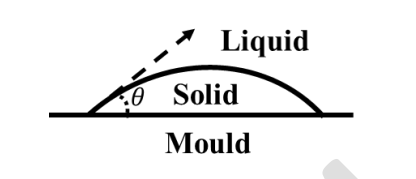
\includegraphics[width=0.3\columnwidth]{figs/Q.33.png}
    \caption\centering{SCHEMATIC DIAGRAM}
    \label{fig:placeholder}
\end{figure}

\item A single crystal is oriented such that the normal to the slip plane makes an angle of $60\degree$ with the tensile axis. If the slip direction makes an angle of $45\degree$ with respect to the tensile axis and the critical resolved shear stress for slip is 2 MPa, then the tensile stress at which plastic deformation commences is \underline{\hspace{2cm}} MPa. (Round off to one decimal place) \hfill{\brak{\text{GATE MT 2024}}}

\item The extrusion force required to extrude an aluminum rod of cross-sectional area of 150 $mm^2$ to cross-sectional area of 50 $mm^2$ is \underline{\hspace{2cm}} N. (Round off to the nearest integer) \hfill{\brak{\text{GATE MT 2024}}}\\
Assume that the extrusion constant, which accounts for the flow stress, strain hardening, friction and inhomogeneous deformation, is equal to 2 MPa.

\end{enumerate}

\subsection*{Q.36 - Q.65 Carry TWO marks Each}
\begin{enumerate}[resume]
\item If

\begin{align}
\myvec{ 1 & 2 \\ 8 & 1 } \myvec{ x \\ y } = \lambda\myvec{ x \\ y}
\end{align}

where $x, y$ are not identically zero, then the values of $\lambda$ are \hfill{\brak{\text{GATE MT 2024}}}
\begin{multicols}{4}
\begin{enumerate}
\item 5, -3
\item 4, -4
\item 3, -5
\item 5, -4
\end{enumerate}
\end{multicols}

\item If $\frac{dy}{dx} = 4xy$, $y(0) = 1$, then \hfill{\brak{\text{GATE MT 2024}}}
\begin{multicols}{2}
\begin{enumerate}
\item $y = 2x^2 + 1$
\item $y = 2e^{2x^2} - 1$
\item $y = 2e^{x^2} - 1$
\item $y = e^{2x^2}$
\end{enumerate}
\end{multicols}

\item As shown in the figure, the right end of a slender, long solid cylindrical metal rod of thermal conductivity $k$, length $L$ and diameter $d (\ll L)$ is in contact with an infinite liquid heat sink. At steady-state, the temperatures of the right end of the rod and the heat sink are $T_2$ and $T_0$, respectively. If the convection heat transfer coefficient between the liquid heat sink and the right end of the rod is $h$, then what would be the temperature of the left end of the rod, $T_1$, at steady-state? Assume that there is no other heat loss. \hfill{\brak{\text{GATE MT 2024}}}
\begin{figure}[H]
    \centering
    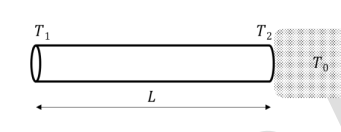
\includegraphics[width=0.4\columnwidth]{figs/Q.38.png}
    \caption\centering{SOLID CYLINDRICAL ROD}
    \label{fig:placeholder}
\end{figure}
\begin{multicols}{2}
\begin{enumerate}
\item $T_1 = T_2 + (T_2 - T_0)\frac{hL}{k}$
\item $T_1 = T_2 - (T_2 - T_0)\frac{hL}{k}$
\item $T_1 = T_2 - (T_2 - T_0)\frac{k}{hL}$
\item $T_1 = T_2 + (T_2 - T_0)\frac{k}{hL}$
\end{enumerate}
\end{multicols}

\item Match the dimensionless numbers listed in Column I with their applications to transport phenomena listed in Column II. \hfill{\brak{\text{GATE MT 2024}}}
\begin{center}
\begin{tabular}{ll}
\textbf{Column I} & \textbf{Column II} \\
P. Reynolds number & 1. Momentum and mass transfer \\
Q. Schmidt number & 2. Momentum and heat transfer \\
R. Prandtl number & 3. Convective and conductive heat transfer \\
S. Biot number & 4. Laminar to turbulent flow \\
\end{tabular}
\end{center}
\begin{multicols}{2}
    \begin{enumerate}
\item P-4, Q-1, R-3, S-2
\item P-3, Q-2, R-4, S-1
\item P-4, Q-1, R-2, S-3
\item P-2, Q-3, R-1, S-4
\end{enumerate}
\end{multicols}

\item In a cubic lattice, what is the ratio of interplanar spacings of the (100), (110) and (111) planes? \hfill{\brak{\text{GATE MT 2024}}}
\begin{multicols}{2}
\begin{enumerate}
\item 1 : 0.32 : 0.71
\item 1 : 0.71 : 0.58
\item 1 : 0.58 : 0.71
\item 1 : 0.58 : 0.32
\end{enumerate}
\end{multicols}

\item The constitutional undercooling condition for a hypothetical binary alloy of A with solute B during solidification is shown in the figure along with its binary phase diagram. Based on these two schematics, one can conclude that the solute concentration in region X will be \underline{\hspace{2cm}} the average composition of the initial liquid phase. \hfill{\brak{\text{GATE MT 2024}}}
\begin{figure}[H]
    \centering
    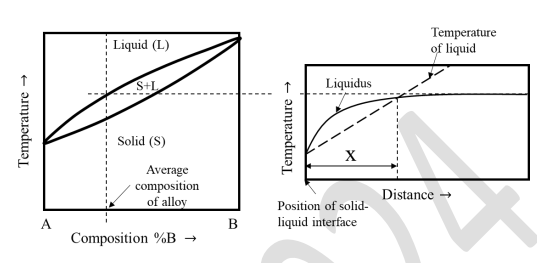
\includegraphics[width=0.6\columnwidth]{figs/Q.41.png}
    \caption\centering{FIGURE}
    \label{fig:labelholder}
\end{figure}
\begin{multicols}{2}

\begin{enumerate}
\item less than
\item greater than
\item same as
\item independent of
\end{enumerate}
\end{multicols}

\item The microstructures of a quenched steel tempered at three temperatures $T_1 < T_2 < T_3$ for a fixed time are schematically illustrated. The solid circles represent cementite particles in ferrite matrix; $\bar{r}_1, \bar{r}_2$ and $\bar{r}_3$ are average radii of cementite particles, and $V_1, V_2$ and $V_3$ are volume fractions of cementite at temperatures $T_1, T_2$ and $T_3$, respectively. If the cementite in steel is more noble than ferrite, then which one of the three microstructures will have the highest corrosion rate when exposed to an aqueous solution of 3.5 wt.\% NaCl? \hfill{\brak{\text{GATE MT 2024}}}
\begin{figure}[H]
    \centering
    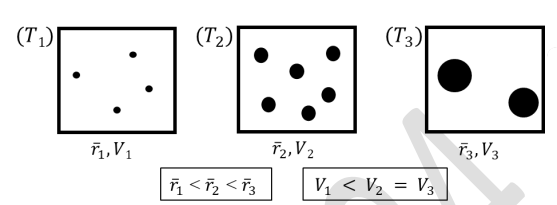
\includegraphics[width=0.6\columnwidth]{figs/Q.42.png}
    \caption\centering{MICROSTRUCTURE OF QUENCHED STEEL}
    \label{fig:placeholder}
\end{figure}
\begin{enumerate}
\item Microstructure at $T_1$
\item Microstructure at $T_2$
\item Microstructure at $T_3$
\item Independent of microstructure
\end{enumerate}

\item An isotropic metallic cuboid block shown in the figure has a coefficient of linear thermal expansion $\alpha$, Young's modulus $E$ and Poisson's ratio $\nu$. The dimensions of the cuboid are $a, b$ and $c$ in the X, Y and Z directions, respectively. It is rigidly constrained against expansion in the X direction. However, it is free to expand in the Y and Z directions. It is initially stress-free. Subsequently, it is heated so that its temperature increases by $\Delta T$. What would be the CHANGE in the dimension of the cuboid in the Y direction? Assume linear elasticity, and that thermal as well as mechanical strains are infinitesimally small. \hfill{\brak{\text{GATE MT 2024}}}
\begin{figure}[H]
    \centering
    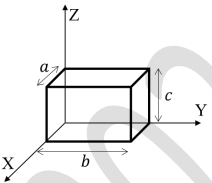
\includegraphics[width=0.3\columnwidth]{figs/Q.43.png}
    \caption\centering{CUBOID}
    \label{fig:placeholder}
\end{figure}
\begin{multicols}{2}
\begin{enumerate}
\item $b(1 - \nu)\alpha\Delta T$
\item $b(1 + \nu)\alpha\Delta T$
\item $b\alpha\Delta T$
\item $b(1 + \alpha)\Delta T$
\end{enumerate}
\end{multicols}

\item Match the entries in Column I with the stacking sequences of the close-packed planes listed in Column II. \hfill{\brak{\text{GATE MT 2024}}}
\begin{center}
\begin{tabular}{ll}
\textbf{Column I} & \textbf{Column II} \\
P. Face centered cubic (FCC) structure & 1. ABCABABC \\
Q. Intrinsic stacking fault in FCC & 2. ABABABAB \\
R. Across an annealing twin boundary in FCC & 3. ABCABCABC \\
S. Hexagonal close-packed structure & 4. ABCABCACBACBA \\
\end{tabular}
\end{center}
\begin{multicols}{2}

\begin{enumerate}
\item P-1, Q-3, R-4, S-2
\item P-2, Q-3, R-1, S-4
\item P-3, Q-1, R-4, S-2
\item P-2, Q-4, R-1, S-3
\end{enumerate}
\end{multicols}

\item Which one of the following graphs represents Griffith's criterion for the growth of a crack in a brittle isotropic infinitely large plate with a center crack? In the graph, $\Delta SE$ is the magnitude of the total strain energy released (shown by solid curve) and $\Gamma_s$ is the total surface energy (shown by dashed line) and $a_c$ is the critical crack length (shown by downward arrow) at which the crack starts growing. The tangent to the $\Delta SE$ curve parallel to the $\Gamma_s$ line is shown by the dotted line. \hfill{\brak{\text{GATE MT 2024}}}
\begin{figure}[H]
    \centering
    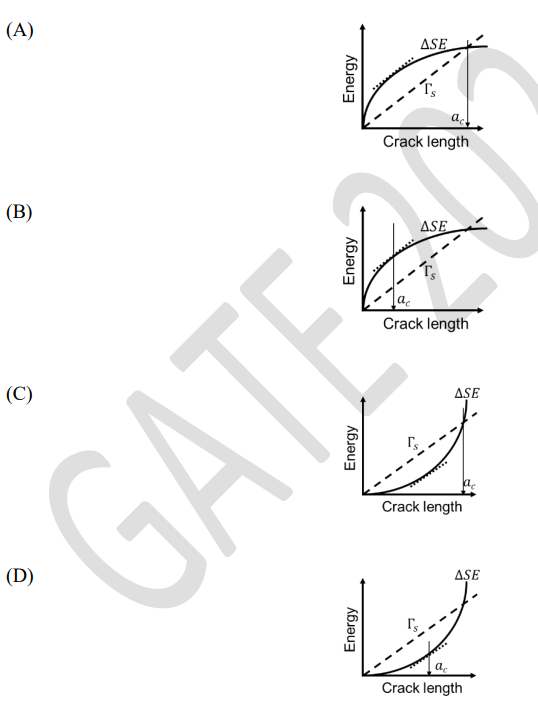
\includegraphics[width=0.6\columnwidth]{figs/Q.45.png}
    \caption\centering{GRAPHS}
    \label{fig:placeholder}
\end{figure}



\item For rolling of slabs, determine the correctness or otherwise of the following Assertion [a] and Reason [r]. \hfill{\brak{\text{GATE MT 2024}}} \\
\textbf{Assertion [a]:} Grooves are made on the surface of the rolls parallel to their roll axes to achieve large thickness reduction in a short time. \\
\textbf{Reason [r]:} Given $\mu$ is the coefficient of friction between the rolls and the slab, and $\alpha$ is the angle of bite between the entrance plane and the centerline of the rolls, unaided entry of slab in the rolls can take place only if $\mu < \tan \alpha$.
\begin{enumerate}
\item Both [a] and [r] are true, and [r] is the correct reason of [a].
\item Both [a] and [r] are true, but [r] is not the correct reason of [a].
\item Both [a] and [r] are false.
\item Statement [a] is true, but [r] is false.
\end{enumerate}

\item Which of the following statements is/are correct?  \hfill{\brak{\text{GATE MT 2024}}}
\begin{enumerate}
\item Ultimate analysis of coal involves determination of moisture, volatile matter, fixed carbon and ash.
\item Reduction of wustite in blast furnace occurs at the lower part of the stack.
\item Roasting involves reduction of sulfide ores to pure metals.
\item White metal (impure \ce{Cu2S}) is produced by oxidizing Fe and S during smelting of Cu-Fe matte.
\end{enumerate}

\item A creep test of a pure polycrystalline metal is performed in tension and the creep strain rate is observed to decrease during the primary stage. The creep mechanism is later determined to be dislocation-climb-controlled. The observed decrease in creep strain rate is/are due to  \hfill{\brak{\text{GATE MT 2024}}}
\begin{enumerate}
\item an increase in dislocation density.
\item grain growth.
\item a decrease in the dislocation density.
\item an increase in the cross-sectional area of the sample.
\end{enumerate}

\item Which of the following statements is/are correct for joining processes?  \hfill{\brak{\text{GATE MT 2024}}}
\begin{enumerate}
\item In case of soldering and brazing, the filler material has a melting point lower than that of the metals joined.
\item In tungsten inert gas welding, tungsten is the filler material.
\item Friction welding is a solid-state joining process.
\item The following reaction is associated with thermit welding:\\
$ C_2H_2(g) + \frac{5}{2} O_2(g)\rightarrow 2CO_2(g) + H_2O(g) + \text{Heat} (\Delta H)$.
\end{enumerate}

\item Which of the following statements is/are correct for non-destructive testing?   \hfill{\brak{\text{GATE MT 2024}}}
\begin{enumerate}
\item Liquid dye penetration technique can be utilized for detecting surface cracks.
\item In radiographic examination, internal cracks cannot be detected.
\item Eddy current-based techniques can be used for detecting sub-surface defects in pure alumina at room temperature.
\item Ultrasonic inspection is unsuitable for inspecting sub-surface defects in high damping capacity material (e.g., cast iron).
\end{enumerate}

\item The following data is obtained from an experiment:
\begin{center}
\begin{tabular}{|c|c|c|c|}
\hline
x & 1 & 2 & 3 \\ \hline
y & 8 & 15 & 19\\
\hline
\end{tabular}
\end{center}
If the data is fit using the straight line $y=mx+c$ (where m and c are constants) using the least-squares method, then the value of m is \underline{\hspace{2cm}}. (Round off to one decimal place). \hfill{\brak{\text{GATE MT 2024}}}

\item The integral $\int_0^1 x e^{-x} dx$ evaluates to \underline{\hspace{2cm}}. (Round off to two decimal places) \hfill{\brak{\text{GATE MT 2024}}}

\item If for element A, the formation enthalpy and formation entropy per vacancy created are 0.5 eV and $3k_B$, respectively, then the equilibrium vacancy concentration (in mole fraction) at 500 K is \underline{\hspace{2cm}} $\times 10^{-4}$. (Round off to two decimal places) \hfill{\brak{\text{GATE MT 2024}}}\\
Given: Boltzmann constant, $k_B = 8.62 \times 10^{-5}\; eV \cdot atom^{-1} \cdot K^{-1}$

\item A steel bar is subjected to fatigue loading with a tensile mean stress. Given that the ultimate tensile strength is 1000 MPa and the fatigue limit under fully reversed loading is 250 MPa, the fatigue limit for a mean stress of 100 MPa, considering Goodman relationship is \underline{\hspace{2cm}} MPa. (Round off to the nearest integer) \hfill{\brak{\text{GATE MT 2024}}}

\item During carburization of a steel at 950$\degree$C, carbon concentration is measured as $0.8 wt.\%$ at a depth of 0.3 mm after one hour. The time required to get the same carbon concentration at a depth of 0.6 mm at the same carburization temperature is \underline{\hspace{2cm}} hours. (Round off to the nearest integer). \hfill{\brak{\text{GATE MT 2024}}}

\item An ideal solution is formed by mixing 10 grams of A and 50 grams of B at 673 K. The molar free energy of mixing \underline{\hspace{2cm}} $kJ.mol^{-1}$. (Round off to one decimal place) \hfill{\brak{\text{GATE MT 2024}}}\\
Given: Universal gas constant $R = 8.314\; J.mol^{-1}.K^{-1}$ \\
Atomic weight of A = 40 $grams.mol^{-1}$ \\
Atomic weight of B = 60 $grams.mol^{-1}$

\item The cupric ion ($Cu^{2+}$) concentration in the electrolyte (at 298 K) required to make the potential of pure copper equal to 0.17 V is \underline{\hspace{2cm}} $\times 10^{-6}\; gram-mol \cdot (litre)^{-1}$. (Round off to two decimal places). \hfill{\brak{\text{GATE MT 2024}}}\\
Gas constant $R = 8.314\; J.mol^{-1}.K^{-1}$ \\
Faraday's constant $F = 96500\; C.mol^{-1}\text{(of electrons)}$ \\
Standard reduction potential of Cu, $E^o = 0.34\; V$

\item A non-porous spherical $Fe_2O_3$ particle of initial radius of $5 \times 10^{-2}\; m$ is topo-chemically reduced by $H_2$, where the reactant-product interface is sharp and spherical, and reaction rate is proportional to the interfacial area. The radius of the unreacted $Fe_2O_3$ particle after 600 s will be \underline{\hspace{2cm}} $\times 10^{-2}\; m$. (Round off to the nearest integer). \hfill{\brak{\text{GATE MT 2024}}}\\
Given: Rate constant $k = 5 \times 10^{-5}\; m.s^{-1}$

\item A long metallic cylindrical rod of radius $r$, length $L (\gg r)$ and electrical resistivity $\rho_e$ is kept in vacuum and is carrying an electric current of $I$. The only way it loses heat to the ambient is via radiation. If the ambient temperature is $T_0$, then the steady-state temperature of the rod is \underline{\hspace{2cm}} K. (Round off to the nearest integer). \hfill{\brak{\text{GATE MT 2024}}}\\
Given: Stefan-Boltzmann constant = $5.667 \times 10^{-8}\; W.m^{-2}.K^{-4}$ \\
$r = 0.1\; mm$, $L = 1\; m$, $\rho_e = 10^{-8}\; \Omega.m$ ,
$I = 0.3\; A$, $T_0 = 300\; K$ \\
Neglect the heat loss by the two flat ends of the rod and assume emissivity = 1.

\item 1000 kg of sphalerite concentrate containing $60\%$ ZnS is COMPLETELY roasted with stoichiometric amount of pure oxygen. The amount of oxygen required is \underline{\hspace{2cm}} kg. (Round off to one decimal place). \hfill{\brak{\text{GATE MT 2024}}}\\
Assume that the other components in the concentrate are not reactive. \\
Given: Atomic weight values (in $gram.mol^{-1}$) for Zn = 65, S = 32, O = 16.

\item 800 grams of A-B alloy containing $20 wt.\%$ B is held at temperature $T_1$. The weight of B dissolved in $\alpha$ at that temperature is \underline{\hspace{2cm}} grams. (Round off to the nearest integer). \hfill{\brak{\text{GATE MT 2024}}}
\begin{figure}[H]
    \centering
    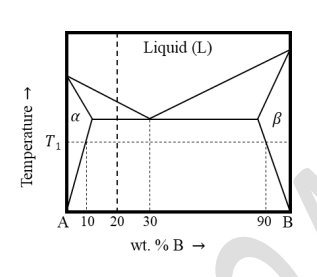
\includegraphics[width=0.5\columnwidth]{figs/Q.61.png}
    \caption\centering{GRAPH}
    \label{fig:placeholder}
\end{figure}

\item A mild steel pipeline is connected to zinc for cathodic protection at a current density of $10\; mA.m^{-2}$. The quantity of zinc required per square meter of the pipeline per year is \underline{\hspace{2cm}} grams. (Round off to the nearest integer). \hfill{\brak{\text{GATE MT 2024}}}\\
Given: Atomic weight of Zn is 65 $gram.mol^{-1}$. \\
Faraday's constant $F = 96500\; C.mol^{-1}\text{(of electrons)}$

\item A large rectangular component is undergoing fully-reversed cyclic loading, and the component is known to grow the dominant fatigue crack from the outer surface. If the stress amplitude ($\sigma_A$) is 100 MPa and the critical stress intensity factor $K_{IC}$ of the material is $50\; MPa.m^{\frac{1}{2}}$ then the crack length at which the component will fail catastrophically is \underline{\hspace{2cm}} mm. (Round off to one decimal place) \hfill{\brak{\text{GATE MT 2024}}}\\
Given: The geometric factor $\alpha$ for this loading condition is 1.12.

\item In casting, for a simple vertical gating system with a gate of cross-sectional area 2 $cm^2$ and sprue height of 10 cm, the filling time for a mould of dimensions $40\; cm \times 20\; cm \times 10\; cm$, is \underline{\hspace{2cm}} s. (Round off to one decimal place) \hfill{\brak{\text{GATE MT 2024}}}\\
Given: Acceleration due to gravity $g = 980\; cm.s^{-2}$

\item During arc welding, the actual heat input is $200\; J.mm^{-3}$ and the current and voltage are 200 A and 20 V, respectively. For a weld cross-sectional area of 2 $mm^2$ and heat transfer efficiency of 0.9, the velocity of welding is \underline{\hspace{2cm}} $mm.s^{-1}$. (Round off to the nearest integer). \hfill{\brak{\text{GATE MT 2024}}}

\end{enumerate}

\section*{*END OF THE QUESTION PAPER*}
 
\end{document}